\section{Introducción}

En el presente trabajo práctico se demuestra que el \textit{Hitting-Set
Problem} como problema de decisión es NP-Completo, se desarrolla una solución
con un algoritmo de \textit{Backtracking} para el mismo, como problema de
optimización, y se analizan posibles soluciones aproximadas.

\section{Definición del \textit{Hitting-Set Problem}}

Dado un conjunto de elemento $A$ de $n$ elementos, $m$ subconjuntos $B_1, B_2,
\ldots, B_m$ de $A \ (B_i \subseteq A \\ \forall \ i)$, queremos el subconjunto
$C \subseteq A$ de menor tamaño tal que $C$ tenga al menos un elemento de cada
$B_i$ (es decir, $C \cap B_i \ne \emptyset$).

\subsection{Como problema de decisión}

Dado un conjunto de elemento $A$ de $n$ elementos, $m$ subconjuntos $B_1, B_2,
\ldots, B_m$ de $A \ (B_i \subseteq A \\ \forall \ i)$, y un número $k$, ¿existe un
subconjunto $C \subseteq A$ con $|C| \le k$ tal que $C$ tenga al menos un
elemento de cada $B_i$ (es decir, $C \cap B_i \ne \emptyset$)?

\section{Demostraciones}

Un problema de decisión $P$ es \textit{NP}-Completo si $P$ pertenece a
\textit{NP} y $P$ es \textit{NP}-Difícil.

\subsection{\textit{Hitting-Set Problem} está en \textit{NP}}

Un problema pertence a $NP$ si una solución al mismo puede ser verificada en
tiempo polinomial por una máquina de Turing determinística, o alternativamente,
el problema puede ser resuelto en tiempo polinomial por una máquina de Turing
no determinística.

El siguiente algoritmo es un posible verificador de soluciones del
\textit{Hitting-Set Problem}:

\lstinputlisting[language=Python]{code/verify.py}

El algoritmo es de tiempo polinomial porque $|B| = m$, $B_i \subseteq A \
\forall \ i$ y $C \subseteq A$, por lo que $|B_i| \le |A|$ y $|C| \le |A|$ y la
complejidad es $\mathcal{O}(N^2m)$ con $N = |A|$. Esto es porque la complejidad
del verificador esta dada por la mayor de las siguientes:

\begin{itemize}
    \item una comparación del tamaño de $C$ contra $k$ ($\mathcal{O}(1)$).

    \item un loop por todos los elementos de $C$ verificando que esten en $A$
    ($\mathcal{O}(N^2)$).

    \item un loop por $m$ elementos (la cantidad de subsets), con otro loop
    adentro de a lo sumo $N$ elementos cada uno (la cantidad de elementos en
    $B_i$) que chequea si algún elemento esta en $C$ (de tamaño a lo sumo $N$),
    que si $C$ es una lista es una operación de tiempo lineal
    ($\mathcal{O}(N^2m)$).
\end{itemize}

\subsection{\textit{Hitting-Set Problem} es \textit{NP}-Difícil}

Para demostrar que el problema es \textit{NP}-Difícil realizamos una reducción
polinomial de un problema \textit{NP}-Completo a nuestro problema,
\href{https://en.wikipedia.org/wiki/Vertex_cover}{\underline{Vertex Cover}}.

Un \textit{Vertex Cover} $V'$ de un grafo no dirigido $G = (V, E)$, es un
conjunto de vertices $V' \subseteq V$, tal que para toda arista $(u, v) \in E$,
$u \in V'\ \lor\ v \in V'$, o lo que es lo mismo, todas las aristas del grafo
$G$ tienen por lo menos una esquina en $V'$. La versión de decisión del
problema se trata de determinar si existe un \textit{Vertex Cover} de a lo sumo
$k$ vértices.

Para reducir este problema al \textit{Hitting-Set Problem} creamos un subset
$B_i = \{ u, v \}$ por cada arista $(u, v) \in E$, $A = V$ y $k = k$. Luego
tomamos la solución del \textit{Hitting-Set Problem} $C$ y con ella generamos
la solución del \textit{Vertex Cover} $V' = C$:

\lstinputlisting[language=Python]{code/vertex_cover.py}

Esta reducción se puede realizar en $\mathcal{O}(V^2)$, que es el costo de
crear un subset por cada arista en el grafo $G$.

\begin{figure}[h]
    \centering
    \begin{subfigure}{0.4\textwidth}
        \centering
        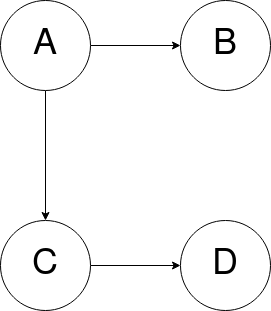
\includegraphics[width=0.585\linewidth]{img/vertex-cover.png}
        \caption{Input de \textit{Vertex Cover}}
    \end{subfigure}
    \begin{subfigure}{0.4\textwidth}
        \centering
        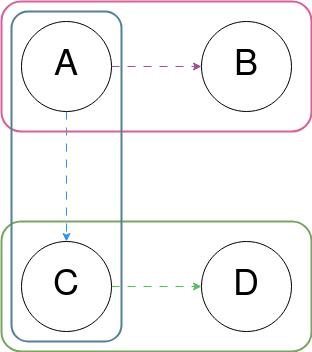
\includegraphics[width=0.6\linewidth]{img/hitting-set.png}
        \caption{Input de \textit{Hitting-Set}}
    \end{subfigure}
    \caption{Reducción de \textit{Vertex Cover} a \textit{Hitting-Set Problem}}
\end{figure}

En el caso de la figura, al generar un set con los dos vértices que componen a
cada una de las aristas, el problema de \textit{Vertex Cover} para el grafo dado
se vería reducido al \textit{Hitting-Set Problem} para los sets $\{A,B\}$,
$\{A,C\}$ y $\{C,D\}$.

Se puede comprobar que el conjunto de soluciones para el \textit{Hitting-Set Problem}
es $\{\{A,D\},\{A,C\},\{C,B\}\}$, que no es ni más ni menos que el conjunto de
soluciones para \textit{Vertex Cover}.